% Тут используется класс, установленный на сервере Papeeria. На случай, если
% текст понадобится редактировать где-то в другом месте, рядом лежит файл matmex-diploma-custom.cls
% который в момент своего создания был идентичен классу, установленному на сервере.
% Для того, чтобы им воспользоваться, замените matmex-diploma на matmex-diploma-custom
% Если вы работаете исключительно в Papeeria то мы настоятельно рекомендуем пользоваться
% классом matmex-diploma, поскольку он будет автоматически обновляться по мере внесения корректив
%
\documentclass{matmex-diploma}
\usepackage{algpseudocode}
\usepackage{algorithm}
\usepackage{caption}
\usepackage{algorithmicx}
\usepackage{amssymb}

\begin{document}

\algtext*{EndWhile}% Remove "end while" text
\algtext*{EndIf}% Remove "end if" text
\algtext*{EndFor}% Remove "end for" text
\algtext*{EndFunction}% Remove "end function" text

% Год, город, название университета и факультета предопределены,
% но можно и поменять.
% Если англоязычная титульная страница не нужна, то ее можно просто удалить.
\filltitle{ru}{
    chair              = {Кафедра системного программирования},
    title              = {Синтаксический анализ регулярных множеств},
    type               = {diploma},
    position           = {студентка},
    group              = 544,
    author             = {Вербицкая Екатерина Андреевна},
    supervisorPosition = {ст. пр., магистр информационных технологий},
    supervisor         = {Григорьев С.\,B.},
    reviewerPosition   = {программист ООО "ИнтеллиДжей Лабс", \\магистр прикладной математики и информатики},
    reviewer           = {Бреслав А.\,А.},
    chairHeadPosition  = {д.\,ф.-м.\,н., профессор},
    chairHead          = {Терехов А.\,Н.},
    city               = {Санкт-Петербург},
    year               = {2015}
}
\filltitle{en}{
    chair              = {Chair of Software Engineering},
    title              = {Parsing of Regular Sets},
    author             = {Ekaterina Verbitskaia},
    supervisorPosition = {Senior Lecturer},
    supervisor         = {Semen Grigorev},
    reviewerPosition   = {Software Developer at IntelliJ Labs},
    reviewer           = {Andrey Breslav},
    chairHeadPosition  = {Professor},
    chairHead          = {Andrey Terekhov},
}
\maketitle
\tableofcontents

\section{Introduction}

Graph querying is finding all paths in the graph which satisfy some constraints.
If the constraints are specified with some language formalism, i.e. a grammar, it is called a language-constrained path query. The simplest query described with a grammar $S \rightarrow a \ b$ being run against the graph in the Fig.~\ref{fig:exmplInputGraph} returns the only path $2, 3, 4$ (shown in red).

A grammar $S \rightarrow a \ S \ b \mid a \ b$ is a query for the paths of the form $a^n b^n$, where $n \geq 1$.
Querying the graph in the Fig.~\ref{fig:exmplInputGraph} returns the infinite set of paths one of which starts and ends in the vertex $3$ and goes around the cycles in the graph the appropriate number of times: $3,1,2,3,1,2,3,4,3,4,3,4,3$.

\begin{figure}[h]
\begin{tikzpicture}[shorten >=1pt,node distance=2cm,on grid,auto]
   \node[state] (q_1)   {$1$};
   \node[state] (q_2) [above=of q_1] {$2$};
   \node[state] (q_3) [above right=of q_1, below right=of q_2] {$3$};
   \node[state] (q_4) [right=of q_3] {$4$};
    \path[->]
    (q_1) edge  node {a} (q_2)
    (q_2) edge[red]  node {a} (q_3)
    (q_3) edge  node {a} (q_1)
    (q_3) edge[bend left, above, red]  node {b} (q_4)
    (q_4) edge[bend left, below]  node {b} (q_3);
\end{tikzpicture}
\caption{An example of input graph}
\label{fig:exmplInputGraph}
\end{figure}

Most existing graph traversing/querying languages, including SPARQL~\cite{sparql}, Cypher~\footnote{Cypher language web page: \url{https://neo4j.com/developer/cypher-query-language/}. Access date: 16.01.2018}, and Gremlin~\cite{gremlin} support only regular languages as constrains.
For some applications, regular languages are not expressive enough.
Context-free path queries (CFPQ), on which we focus this paper, employ context-free languages for constraints specification.
CFPQs are used in bioinformatics~\cite{GraphQueryWithEarley}, static code analysis~\cite{Reps, Zheng, LabelFlowCFLReachability, specificationCFLReachability, JavaCFL}, and RDF processing~\cite{CFGonRDF}.
Although there is a lot of problem-specific solutions and theoretical research on CFPQs~\cite{Yannakakis, ConjCFPathQuery, Hellings16, GrigorevR16, QueryGraphWithData, RegularDBQuery, GraphQueryWithEarley, graphDB}, cfSPARQL~\cite{CFGonRDF} is the single known graph query language to support CF constraints.
Generic solution for the integration of CFPQs into general-purpose languages is not discussed enough.

When developing a data-centric application, one wants to use a general-purpose programming language and also to have transparent and native access to data sources.
One way to achieve this is to use string-embedded DSLs.
In this approach, a query is written as a string, then passed on to a dedicated driver which executes it and returns a possibly untyped result.
Despite the simplicity, string-embedded DSLs have serious drawbacks.
First of all, they require the developer to learn the language itself, its features, runtime, and how the integration between the languages is implemented.
DSLs are also a source of possible errors and vulnerabilities, static detection of which is a serious challenge~\cite{stringEmbeddedLanguagesProblem}.
Such techniques as the Object Relationship Mapping (ORM) or Language Integrated Query~(LINQ)~\cite{LINQ1, LINQ2, LinqRDF} partially solve these problems, but they still have issues with flexibility: both query decomposition and  reusing of subqueries are a struggle.
In this paper, we propose a transparent and natural integration of CFPQs into a general-purpose programming language.

Context-free path queries are known in various domains under different names. The \emph{context-free language reachability framework} or  \emph{IFDS framework} is how they are called in the area of static code analysis.
In~\cite{Reps:1995, Reps} Thomas Reps shows that the wide range of static code analysis problems can be formulated in terms of CFL-reachability in the graph.
This framework is used for such problems as the taint analysis~\cite{CFLTaint}, the alias analysis~\cite{JavaCFL, Zheng, CFLGraspan}, the label flow analysis~\cite{LabelFlowCFLReachability}, and the fix locations problem~\cite{CFLfinding}.
What we propose in the paper can be viewed as a core of such framework since it provides both problem and domain independent mechanism for CFPQ evaluation.

We view parser combinators as the best way to integrate context-free language specifications into a general-purpose programming language. Parser combinators provide not only a transparent integration but also compile-time checks of correctness and high-level techniques for generalization. An idea to use combinators for graph traversing has already been proposed in~\cite{ScalaGraphParsing}. Unfortunately, the solution presented processes cycles in the input graph only approximately and is unable to handle left-recursive combinators, which is the most common issue of the approach. Authors pointed out that the idea described is similar to the parser combinators, but the language class supported or restrictions are not discussed.

Parser combinators are known to handle only a subset of context-free grammars: left recursion and ambiguity of the grammars are problematic.
In~\cite{Meerkat}, the authors demonstrate a set of parser combinators which handles arbitrary context-free grammars by using ideas of the Generalized LL~\cite{scott2010gll} algorithm (GLL).
Meerkat~\footnote{Meerkat project repository:~\url{https://github.com/meerkat-parser/Meerkat}. Access date: 16.01.2018} parser combinators library implements the ideas from the paper~\cite{Meerkat} and provides the parsing result in a compact form as a Shared Packed Parse Forest~\cite{SPPF}~(SPPF).
SPPF is a suitable finite structural representation of a CFPQ result, even when the set of paths is infinite~\cite{GrigorevR16}.
All the paths can be extracted from the SPPF---in the form of the corresponding derivation trees---and further analysis can be done.
It is also possible to run some further processing over the SPPF itself---not extracting the paths explicitly.

In this paper, we compose these ideas and present a set of parser combinators for context-free path querying which handles arbitrary context-free grammars and provides a structural representation of the result.
We make the following contributions in the paper.

\begin{enumerate}
\item We show that it is possible to create a set of parser combinators for context-free path querying which works on both arbitrary context-free grammars and arbitrary graphs and provides a finite structural representation of the query result.
\item We implement the parser combinators library in Scala. This library provides integration to Neo4j~\footnote{Neo4j graph database site: \url{https://neo4j.com/}. Access date: 16.01.2018} graph database. The source code is available on GitHub: \url{https://github.com/YaccConstructor/Meerkat}.
\item We perform an evaluation on realistic data and compare the performance of our library with another GLL-based CFPQ tool and with the Trails library.
We conclude that our solution is expressive and performant enough to be applied to the real-world problems.
\end{enumerate}

This paper is organized as follows.
We introduce a formal definition of the CFPQ problem in section~\ref{sec:CFPQ}, and we provide a basic description of the Meerkat library and SPPF data structure in section~\ref{sec:GLL}.
We describe our solution in section~\ref{sec:combinators}.
In section~\ref{sec:examples} we present and discuss a set of classical queries (the same generation query, the queries to a movie dataset~\footnote{The movie database is a traditional dataset for graph databases. Detailed description is available here: \url{https://neo4j.com/developer/movie-database/}. Access date: 16.01.2018})
written with our library.
Evaluation of the library is described in section~\ref{sec:evaluation}.
Finally, In section~\ref{sec:conclusion} we conclude and discuss possible directions for further research.

\section{Постановка задачи}
Целью данной работы является разработка алгоритма ослабленного синтаксического 
анализа для регулярной аппроксимации множества значений динамически формируемого
выражения, который для всех корректных относительно некоторой эталонной 
грамматики цепочек строит конечное представление множества деревьев разбора, при
этом цепочки, не принадлежащие эталонному языку, игнорируются.

В рамках данной дипломной работы поставлены следующие задачи.
\begin{itemize}
  \item Разработать алгоритм синтаксического анализа динамически формируемых 
        выражений, поддерживающий работу с произвольными входными графами.
  \item Реализовать предложенный алгоритм.
  \item Доказать корректность алгоритма.
  \item Провести апробацию.
\end{itemize}
\section{Related Works}

Our approach for syntax analysis of string-embedded languages borrows some common principles
from existing techniques in this area. In addition, we reuse RNGLR syntax analysis algorithm 
and some accompanying constructs. In this section we provide a review and recollect some important
notions which will be referred to later on. 

\subsection{String-Embedded Languages Analysis Techniques}
The analysis of string-embedded languages, as a rule, requires a set of \emph{hotspots} to
be indicated in the host application source code. Hotspot is considered as some ``point 
of interest'', where the analysis of the set of possible string values is desirable. This task can be
performed either in a user-assisted manner or automatically using some pragmatic 
considerations or knowledge of the framework being analyzed. The following logical steps 
include static analysis to construct an approximation for the set of all possible string values,
lexical, syntax, and, perhaps, some kind of semantic analysis. These steps are not
necessarily performed separately; some of them may be omitted.

A rather natural idea of \emph{regular approximation} is to approximate the set of all possible 
strings by a regular expression. In recognition-centric formulation, this approach boils down to
the problem of inclusion of approximating regular language into context-free reference language, which
is decidable for a number of practically significant cases~\cite{LangInclusion}.
Many approaches follow this route. In~\cite{Stranger}, forward reachability analysis is used to compute regular 
approximation for all string values in the program. Further analysis is based on patterns detection in approximation 
set or generation of some finite subset of strings for analysis by standalone tools. Regular approximation in~\cite{JSA} 
is acquired by widening context-free approximation, initially built as a result of program analysis. 
Our approach is partially inspired by Alvor~\cite{Alvor,ALVOR2} which utilizes GLR-based technique for syntax 
analysis of regular approximation; this framework implements abstract lexical analysis to convert a
regular language over characters into regular language over tokens, which simplifies syntax analysis.

Kyung-Goo Doh et al. in a series of papers~\cite{AbstrParsing,LRAbstrParsing,LRAbstrParsingSema} introduced an
approach, based on implicit representation of the set of potential strings as a system of data-flow equations. 
Conventional LALR(1) is chosen for the basis of parsing algorithm; original parse tables are reused. 
Syntax analysis is performed as the system of dataflow equations is being solved iteratively in the space of abstract stacks.
The problem of infinite stack growth, which appears in general case, is handled using abstract 
interpretation~\cite{AbstractInterpretation}. This approach later evolved to a certain kind of semantic processing
in terms of attribute grammars which made it possible to analyze a wider class of languages, than
LALR(1).

\subsection{Right-Nulled Generalized LR Parsing Algorithm}
RNGLR (Right-Nulled Generalized LR) is a modification of Generalized LR (GLR) algorithm, which
was developed by Masaru Tomita~\cite{Tomita} in the context of natural language processing. 
GLR was designed to handle ambiguous context-free grammars. Ambiguities in the grammar produce 
shift/reduce and reduce/reduce conflicts, speaking in terms of LR approach. The algorithm 
uses parse tables, similar to those for classical LR, each cell of which can contain multiple 
actions. The general approach is to carry out all possible actions during parsing 
using graph-based data structures to efficiently represent the set of stacks 
and derivation trees. Originally, Tomita's algorithm was unable to recognize all context-free languages.  
Elizabeth Scott and Adrian Johnstone presented RNGLR~\cite{RNGLR},
which extends GLR with a certain way of handling \emph{right nullable} 
rules (i.e. rules of the form $\mathrm{A} \rightarrow \alpha \beta$, where $\beta$ 
reduces to an empty string).

To efficiently represent the set of all stacks produced during parsing,
RNGLR uses Graph Structured Stack (GSS). GSS is a directed graph,
whose vertices correspond to the elements of individual stacks and edges link successive
stack elements. Each vertex can have multiple incoming and outgoing edges to merge 
multiple stacks together; thus stack element sharing is implemented. Each vertex is 
a pair $(s,l)$, where $s$ is a parser state and $l$ is a \emph{level} (position in the input string). 
Vertices in GSS are unique and there are no multi-edges. 

According to RNGLR, an input is read left-to-right, one token at a time, and 
the levels of GSS are constructed sequentially for each input position: first, all  
possible reductions are applied, then the next input terminal is shifted and
pushed to the GSS. When a reduction or pushing is performed, 
the algorithm modifies GSS in the following manner. Suppose an 
edge $(v_t,v_h)$ has to be added to the GSS. By construction, the head vertex
$v_h$ is always already in the GSS. If the tail vertex is also in the GSS, then
a new edge $(v_t,v_h)$ is added (provided it is not yet there); otherwise both 
new tail vertex and new edge are created and added to the GSS. Every time a new 
vertex $v=(s,l)$ is created, the algorithm calculates the new parser 
state $s'$ from $s$ and the next terminal of the input. The pair $(v,s')$, called 
\emph{push}, is added to the global collection $\mathcal{Q}$. The set of $\epsilon$-reductions (i.e. reductions with length $l=0$) 
is also calculated, when a new vertex is added to the GSS, and reductions from this set are added to the 
global queue $\mathcal{R}$. Reductions with length $l>0$ are calculated and added to $\mathcal{R}$ 
each time a new (non-$\epsilon$) edge is created. 

An input string can have several derivation trees and, as a rule, they can have 
numerous identical subtrees. Shared Packed Parse Forest (SPPF)~\cite{SPPF} is a directed graph
designed for a compact representation of all possible derivation trees.  
SPPF has the following structure: the \emph{root} (i.e. vertex with no incoming edges) corresponds 
to the starting nonterminal of the grammar; vertices with no outgoing edges correspond to terminals 
or derivation of $\epsilon$-string; the rest of the vertices is divided into two classes: \emph{nonterminal} 
and \emph{production}. Each nonterminal vertex keeps a collection of production nodes, each of which represents one  
possible derivation of that nonterminal. Production vertices represent a right-hand side of the 
production and keep an ordered list of terminal or nonterminal nodes. The length of this list lies
in the range $[l-k..l]$, where $l$ is the length of production right-hand side, and $k$ is 
the number of rightmost symbols which derive $\epsilon$ (nullable symbols are ignored to reduce memory consumption).

SPPF is constructed simultaneously with GSS. Each edge of the GSS is associated with either 
a terminal or nonterminal node. When a GSS edge is added with a push, 
a new terminal node is created and associated with the edge. Nonterminal nodes are associated
with edges which were added, when reductions were performed: if the edge has already been in GSS, 
a production node is added to the family of nonterminal nodes, associated with the edge. All subgraphs 
from the edges of the reduction path are added as children to the production node. After the input 
is read to the end, all vertices with accepting states are searched and nodes associated with 
outgoing edges of such vertices are merged to form the resulting SPPF. All unreachable vertices 
are deleted from the SPPF graph, which leaves only the actual derivation trees for the input.

The detailed algorithm description in the form of pseudocode can be found in Appendix~\ref{RNGLRCode}.

\clearpage
\setmonofont[Mapping=tex-text]{CMU Typewriter Text}
\section{Алгоритм ослабленного синтаксического анализа регулярной аппроксимации динамически формируемого выражения}

\subsection{Описание алгоритма}
Алгоритм принимает на вход эталонную грамматику $G$ над алфавитом терминальных символов $T$ и детерминированный конечный автомат $(Q,\Sigma,\delta,q_0,q_f)$, имеющий одно стартовое состояние $q_0$, одно конечное состояние $q_f$, без $\epsilon$-переходов, где $\Sigma \subseteq T$~--- алфавит входных символов, $Q$~--- множество состояний, $\delta$~--- отношение перехода. По описанию  грамматики генерируются управляющие RNGLR-таблицы и некоторая вспомогательная информация (называемая $parserSource$ в псевдокоде).

\begin{algorithm}[!ht]
\begin{algorithmic}[1]
\caption{Алгоритм ослабленного синтаксического анализа регулярной аппроксимации динамически формируемого выражения}
\label{parsing}
\Function{parse}{$grammar, automaton$}
  \State{$inputGraph \gets$ construct inner graph representation of $automaton$}
  \State{$parserSource \gets$ generate RNGLR parse tables for $grammar$}
  \If{$inputGraph$ contains no edges}
    \If{$parserSource$ accepts empty input} {report success}
    \Else { report failure}
    \EndIf
  \Else
    \State{\Call{addVertex}{$inputGraph.startVertex, startState$}}
    \State{$\mathcal{Q}.Enqueue(inputGraph.startVertex)$}
    \While{$Q$ is not empty}
      \State{$v \gets \mathcal{Q}.Dequeue()$}
      \State{\Call{makeReductions}{$v$}}
      \State{\Call{push}{$v$}}
      \State{\Call{applyPassingReductions}{$v$}}
    \EndWhile
    \If{$\exists v_f: v_f.level = q_f$ and $v_f.state$ is accepting} {report success}
    \Else { report failure}
    \EndIf
  \EndIf
\EndFunction
\end{algorithmic}
\end{algorithm}

Алгоритм производит обход графа входного автомата и последовательно строит GSS тем же способом, как это делает RNGLR-алгоритм. Однако, так как мы имеем дело с графом вместо линейного потока, понятие следующего символа трансформируется во \emph{множество терминальных символов}, лежащих на всех исходящих рёбрах данной вершины, что несколько изменяет операции shift и reduce (смотри строку 5 в алгоритме~\ref{processVertex} и строки 9 и 21 в алгоритме~\ref{gss_construction}). Для того, чтобы управлять порядком обработки вершин входного графа, мы используем глобальную очередь $\mathcal{Q}$. Каждый раз, когда добавляется новая вершина GSS, сначала необходимо произвести все свёртки длины 0, после чего выполнить сдвиг следующих токенов со входа. Таким образом необходимо добавить соответствующую вершину графа в очередь на обработку. Добавление нового ребра GSS может порождать новые свёртки, таким образом в очередь на обработку необходимо добавить вершину входного графа, которой соответствует начальная вершина добавленного ребра. Детальное описание процесса построения GSS приведено в алгоритме~\ref{parsing}. Свёртки производятся вдоль путей в GSS, и если было добавлено ребро, начальная вершина которого ранее присутствовала в GSS, необходимо заново вычислить проходящие через эту вершину свёртки (смотри функцию applyPassingReductions в алгоритме~\ref{processVertex}).

\begin{algorithm}[H]
\begin{algorithmic}[1]
\caption{Обработка вершины внутреннего графа}
\label{processVertex}
\Function{push}{$innerGraphV$}
  \State{$\mathcal{U} \gets$ copy $innerGraphV.unprocessed$}
  \State{clear $innerGraphV.unprocessed$}
  \ForAll{$v_{h}$ in $\mathcal{U}$}  
    \ForAll{$e$ in outgoing edges of $innerGraphV$}
      \State{$push \gets$ calculate next state by $v_{h}.state$ and the token on $e$}
      \State{\Call{addEdge}{$v_{h}, e.Head, push, false$}}
      \State{add $v_{h}$ in $innerGraphV.processed$}
    \EndFor
  \EndFor
\EndFunction

\Function{makeReductions}{$innerGraphV$}
  \While{$innerGraphV.reductions$ is not empty}
    \State{$(startV, N, l) \gets innerGraphV.reductions.Dequeue()$}
    \State{find the set of vertices $\mathcal{X}$ reachable from $startV$}
    \State{    along the path of length ($l-1$), or $0$ if $l=0$;}
    \State{add $(startV, N, l-i)$ in $v.passingReductions$,}
    \State{    where $v$ is an $i$-th vertex of the path}
    \ForAll{$v_{h}$ in $\mathcal{X}$}
      \State{$state_{t} \gets$ calculate new state by $v_{h}.state$ and nonterminal $N$}
      \State{\Call{addEdge}{$v_{h}, startV, state_{t}, (l=0)$}}
    \EndFor
  \EndWhile
\EndFunction

\Function{applyPassingReductions}{$innerGraphV$}
  \ForAll{$(v, edge)$ in $innerGraphV.passingReductionsToHandle$}
    \ForAll{$(startV, N, l) \gets v.passingReductions.Dequeue()$}
      \State{find the set of vertices $\mathcal{X}$,}
      \State{    reachable from $edge$ along the path of length ($l-1$)}
      \ForAll{$v_{h}$ in $\mathcal{X}$}
        \State{$state_{t} \gets$ calculate new state by $v_{h}.state$ and nonterminal $N$}
        \State{\Call{addEdge}{$v_{h}, startV, state_{t}, false$}}
      \EndFor
    \EndFor
  \EndFor
\EndFunction
\end{algorithmic}
\end{algorithm}

Так же как и RNGLR, мы ассоциируем вершины GSS с позициями входного графа, однако в нашем случае уровень вершины~--- это состояние входного автомата. Мы строим внутреннюю структуру данных (в дальнейшем изложении называемую \emph{внутренним графом}) посредством копирования графа входного автомата и ассоциации с его вершинами следующих коллекций.
\begin{itemize}
  \item \emph{processed}: вершины GSS, для которых ранее были вычислены все операции push. Это множество агрегирует все вершины GSS, ассоциированные с вершиной внутреннего графа.
  \item \emph{unprocessed}: вершины GSS, операции push для которых ещё только предстоит выполнить. Это множество аналогично множеству $\mathcal{Q}$ алгоритма RNGLR.
  \item \emph{reductions}: очередь, аналогичная очереди $\mathcal{R}$ RNGLR-алгоритма: все операции reduce, которые ещё только предстоит выполнить.
  \item \emph{passingReductionsToHandle}: пары из вершины GSS и ребра GSS, вдоль которых необходимо осуществлять проходящие свёртки.
\end{itemize}

\begin{algorithm}[H]
\begin{algorithmic}[1]
\caption{Построение GSS}
\label{gss_construction}
\Function{addVertex}{$innerGraphV, state$}
  \State{$v \gets$ find a vertex with state $=state$ in}
  \State{    $innerGraphV.processed \cup innerGraphV.unprocessed$}
  \If{$v$ is not $null$ } \Comment{Вершина была найдена в GSS}
    \State{\Return{($v, false$)}} 
  \Else
    \State{$v \gets$ create new vertex for $innerGraphV$ with state $state$}
    \State{add $v$ in $innerGraphV.unprocessed$}
    \ForAll{$e$ in outgoing edges of $innerGraphV$}
      \State{calculate the set of zero-reductions by $v$}
      \State{    and the token on $e$ and add them in $innerGraphV.reductions$}
    \EndFor
    \State{\Return{$(v, true$)}}
  \EndIf
\EndFunction

\Function{addEdge}{$v_{h}, innerGraphV, state_{t}, isZeroReduction$}
  \State{$(v_{t}, isNew) \gets$ \Call{addVertex}{$innerGraphV, state_{t}$}}
  \If{GSS does not contain edge from $v_{t}$ to $v_{h}$}
    \State{$edge \gets$ create new edge from $v_{t}$ to $v_{h}$}
    \State{$\mathcal{Q}.Enqueue(innerGraphV)$}
    \If{not $isNew$ and $v_{t}.passingReductions.Count>0$}
      \State{add $(v_{t}, edge)$ in $innerGraphV.passingReductionsToHandle$}
    \EndIf
    \If{not $isZeroReduction$}
      \ForAll{$e$ in outgoing edges of $innerGraphV$}
        \State{calculate the set of reductions by $v$}
        \State{    and the token on $e$ and add them in $innerGraphV.reductions$}
      \EndFor
    \EndIf
  \EndIf
\EndFunction
\end{algorithmic}
\end{algorithm}

Помимо состояния анализатора $state$ и уровня $level$ (который совпадает с состоянием входного автомата), в вершине GSS хранится коллекция \emph{проходящих свёрток}. Проходящая свёртка~--- это тройка $(startV, N, l)$, соответствующая свёртке, чей путь содержит данную вершину GSS. Аналогичная тройка используется в RNGLR-алгоритме для описания свёртки, но в данном случае $l$ обозначает длину оставшейся части пути. Проходящие свёртки сохраняются в каждой вершине пути (кроме первой и последней) во время поиска путей в функции $makeReductions$ (см. алгоритм~\ref{processVertex}).

\subsection{Построение компактного представления леса разбора}
В качестве компактного представления леса разбора всех корректных выражений из множества значений динамически формируемого выражения используется граф SPPF. Построение компактного представления осуществляется одновременно с синтаксическим разбором во время построения графа стеков GSS, также как и в алгоритме RNGLR.

С каждым ребром GSS ассоциируется список лесов разбора фрагмента выражения. В графе GSS нет кратных рёбер, поэтому если во время работы функции \emph{addEdge} в нем было найдено добавляемое ребро, то с ним ассоциируется новый лес разбора, при этом в очередь на обработку не добавляется никаких вершин входного графа.  

При добавлении в GSS ребра, соответствующего считанной со входа лексеме, создаётся (и ассоциируется с ним) граф из одной терминальной вершины. Так как входной автомат является детерминированным, с ребром GSS ассоциируется не более одного такого графа.

При обработке свёртки алгоритм осуществляет поиск всех путей в графе GSS заданной длины, после чего происходит добавление в GSS новых рёбер, соответствующих данной свёртке. С каждым таким ребром ассоциируется лес, имеющий в качестве корня (вершины, у которой нет входных рёбер) вершину, соответствующую нетерминалу, к которому осуществлялась свёртка. Ребра каждого из найденных путей, перечисленные в обратном порядке, образуют правую часть некоторого правила грамматики, по которому осуществляется свёртка. Для каждого пути создаётся вершина, помеченная номером такого правила, и добавляется в лес как непосредственно достижимая из корня. Каждое ребро пути ассоциировано со списком лесов вывода символа из правой части правила. Непосредственно достижимыми вершинами вершины-правила становятся ссылки на такие списки, за счёт чего осуществляется переиспользование фрагментов леса.

В алгоритме RNGLR наличие нескольких путей, вдоль которых осуществляется свёртка к нетерминалу, означает существование более чем одного варианта вывода нетерминала. В нашем случае данная ситуация соответствует различным фрагментам нескольких выражений из входного регулярного множества, которые сворачиваются к одному нетерминалу. 

В конце работы алгоритма осуществляется поиск рёбер GSS, для каждого из которых верно, что конечная вершина имеет уровень, равный финальному состоянию входного автомата, и принимающее состояние (accepting state). Результирующее представление леса разбора получается путём удаления недостижимых вершин из графа, созданного объединением лесов разбора, ассоциированных с найденными рёбрами GSS.

Рассмотрим следующий фрагмент кода, динамически формирующий выражение \emph{expr} в строке 4. 
\begin{verbatim}
1 string expr = "" ;
2 for(int i = 0; i < len; i++) 
3 {
4     expr = "()" + expr;
5 }
\end{verbatim}

Множество значений выражения \emph{expr} аппроксимируется регулярным выражением $(\mbox{\texttt{LBR }} \mbox{\texttt{RBR}})*$, где $\mbox{\texttt{LBR }}$ соответствует открывающейся скобке, а $\mbox{\texttt{RBR}}$~--- закрывающейся. Граф конечного автомата, задающего такую аппроксимацию, изображён на рисунке~\ref{input}.
\begin{figure}[!h]
 \centering
 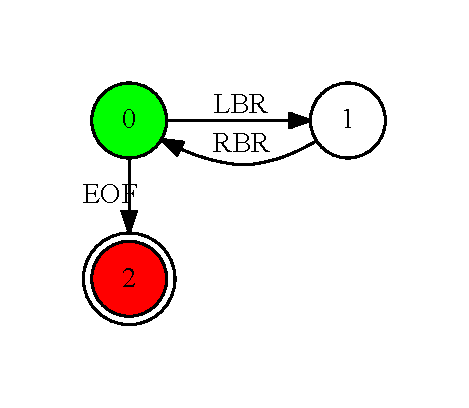
\includegraphics[]{pics/input.pdf}
 \caption{Конечный автомат, задающий регулярную аппроксимацию выражения \emph{expr}}
 \label{input}
\end{figure}

В результате работы предложенного алгоритма будет получено конечное представление леса разбора SPPF, изображённое на рисунке~\ref{sppf}.
\begin{figure}[!h]
 \centering
 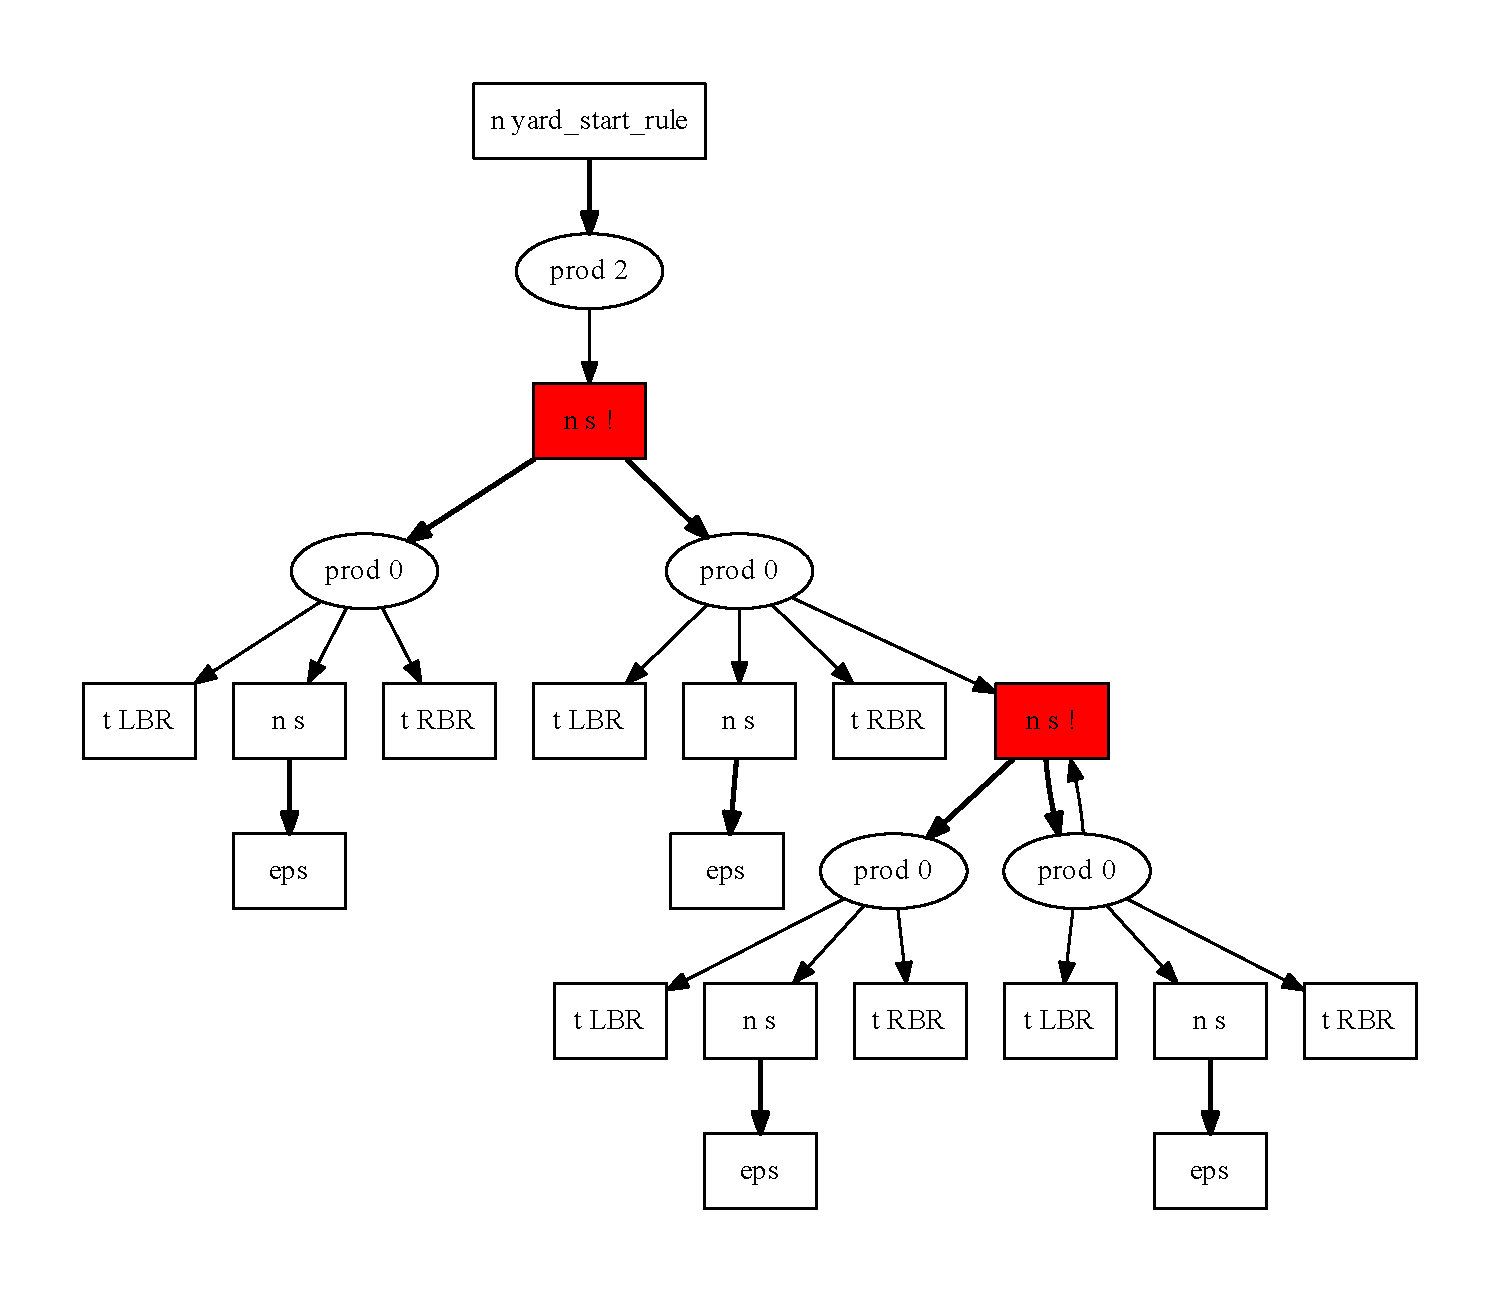
\includegraphics[width=15cm]{pics/sppf.pdf}
 \caption{Конечное представление леса разбора для выражения \emph{expr}}
 \label{sppf}
\end{figure}

%\begin{figure}[!h]
% \centering
% 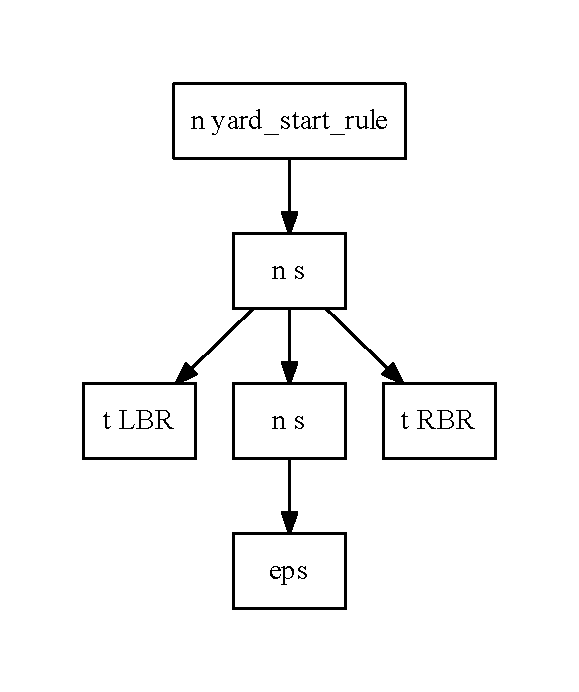
\includegraphics[]{pics/sppf1.pdf}
% \caption{Дерево вывода для выражения $expr="()"$}
% \label{sppf1}
%\end{figure}
%\begin{figure}[!h]
% \centering
% 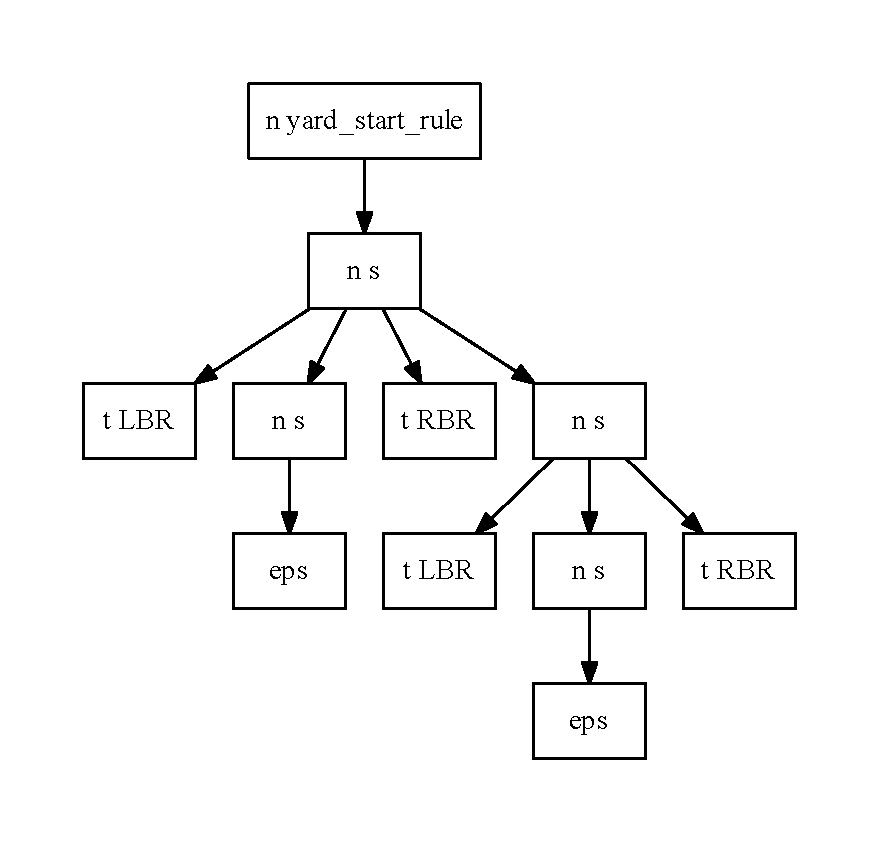
\includegraphics[]{pics/sppf2.pdf}
% \caption{Дерево вывода для выражения $expr="()()"$}
% \label{sppf2}
%\end{figure}
\begin{figure}[!h]
 \centering
 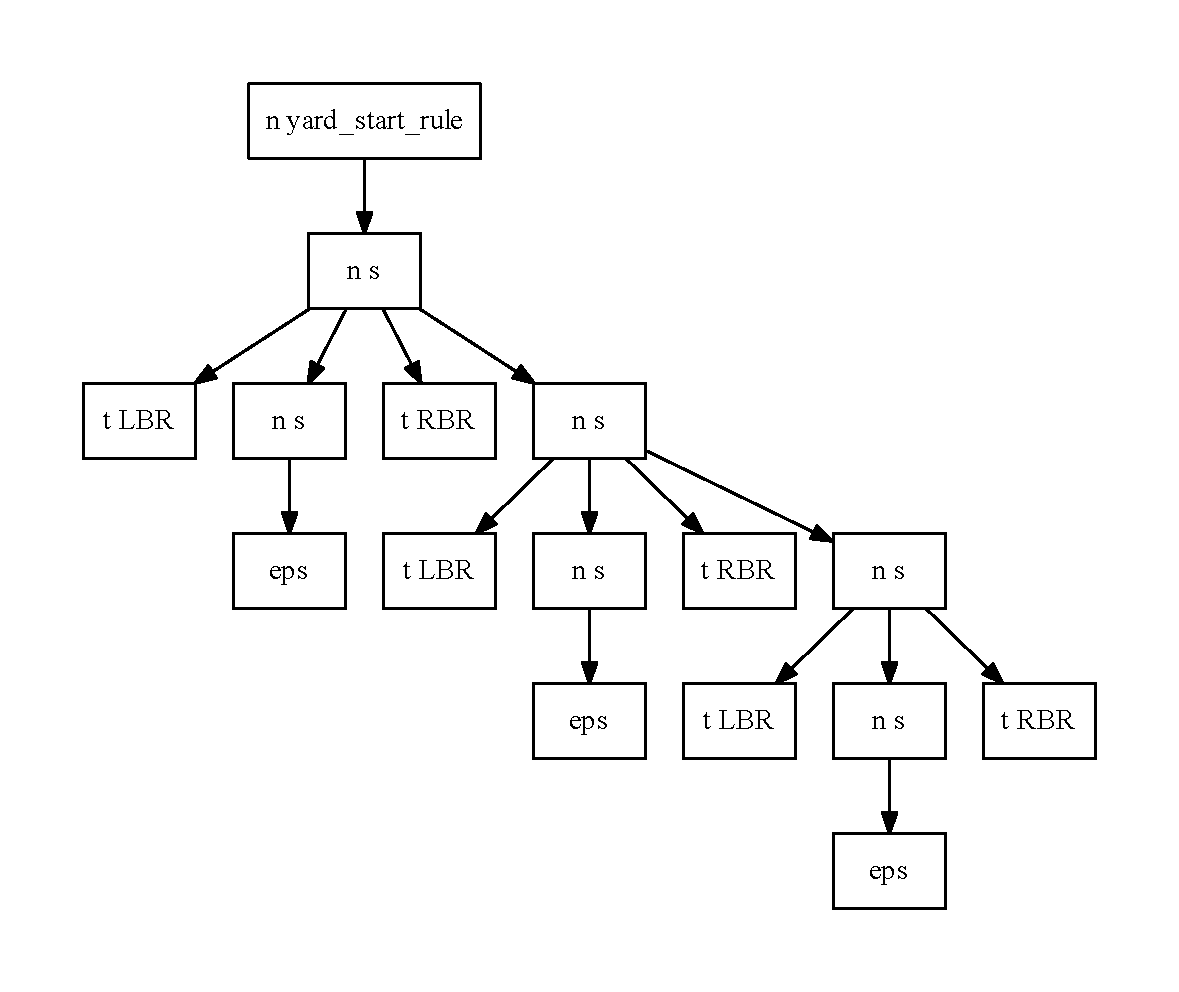
\includegraphics[width=15cm]{pics/sppf3.pdf}
 \caption{Дерево вывода для выражения $expr="()()()"$}
 \label{sppf3}
\end{figure}

Из SPPF можно извлечь бесконечное количество деревьев, каждое из которых является деревом вывода некоторого выражения из регулярной аппроксимации. Рисунок~\ref{sppf3} демонстрирует одно из таких деревьев разбора. 
\section{Correctness of the Algorithm}
In this section we prove the correctness of the algorithm proposed, namely \textsc{Theorem 1} proves its termination,
and \textsc{Theorem 2} and \textsc{Theorem 3} prove correctness of parse forest construction.
In \textsc{Definition}, we slightly redefine classical notion of correct parse tree to better suit our problem. 
SPPF construction is inherited from RNGLR-algorithm, so the proofs are presented
in terms of GSS construction correctness. 

\textsc{Theorem 1.}
\textit{Algorithm terminates for any input.}

\textsc{Proof.}
Each vertex of inner representation of the input finite automaton contains, at most, 
$N$ GSS vertices, where $N$ is a number of parser states. So, the total number of 
GSS vertices is, at most, $N\times n$, where $n$ is the number of vertices in the inner graph. 
Since GSS has no multi-edges, the number of its edges is $O((N\times n)^2)$. The algorithm 
dequeues vertex to be processed from $\mathcal Q$ in the each iteration of the 
main loop. Vertices are enqueued to $\mathcal Q$ only when a new edge is added to GSS. Since the number of 
GSS edges is finite, the algorithm always terminates. \qed

\textsc{Definition.} 
\emph{Correct tree} is an ordered tree with the following properties:
\begin{enumerate}
  \item The root is the start nonterminal of the grammar $G$.
  \item The leaf nodes are terminals of $G$. The sequence of the leaf nodes 
        corresponds to some path in the inner graph. 
  \item The interior nodes are nonterminals of $G$. All children of nonterminal 
        $N$ correspond to the symbols of the right-hand side of some production for $N$ in $G$.
\end{enumerate}

\textsc{Lemma.}
For every GSS edge $(v_{t}, v_{h})$, $v_{t} \in V_{t}.processed$, $v_{h} \in V_{h}.processed$, 
the terminals of the associated subtree correspond to some path in the inner graph $p$ 
from $V_{h}$ to $V_{t}$.

\textsc{Proof.}
The proof is by induction on the height of derivation tree. 
The base case is either some $\epsilon$-tree or a tree with the single leaf. An $\epsilon$-tree corresponds 
to a path of zero length; the tail and the head of the edge associated with $\epsilon$-tree are identical, 
thus the statement is true. A tree with the single leaf corresponds to a single terminal read from an edge 
($V_{h}$, $V_{t}$) of the inner graph, thus the statement is true.

A tree of height $k$ has a nonterminal $N$ as its root. By third statement of correct tree definition, 
there is a production $N \rightarrow A_{0}, A_{1}, \dots, A_{n}$ for children $A_{0}, A_{1}, \dots, A_{n}$ of the root node. 
A subtree $A_{i}$ is associated with GSS edge $(v_{t}^{i}, v_{h}^{i})$ and, as its height is $k-1$, by inductive hypothesis,
there is a path in the inner graph from $V_{h}^{i}$ to $V_{t}^{i}$. $V_{t}^i = V_{h}^{i+1}$, since $v_{t}^i = v_{h}^{i+1}$, 
thus there is a path in the inner graph from $V_{h}^{0}$ to $V_{t}^{n}$, corresponding to the tree under consideration.
\qed

\textsc{Theorem 2.} 
\textit{Every generated from SPPF tree is correct.}

\textsc{Proof.} Consider arbitrary tree, generated from SPPF, and prove that it is correct. The first and the third statements
of correctness definition immediately follow from SPPF definition. 

{\bf (did'not understand the following statement; Russian decryption is required:)}
\textsc{Lemma 1} proves the second item of the definition by consideration of all the edges from the GSS vertex
on the last level having accepting state to the vertex on the 0-level with the start parser state.

\qed

\textsc{Theorem 3.} 
\textit{For every path $p$ in the inner graph, a correct tree corresponding to $p$ can be generated from SPPF.}

\textsc{Proof.}
Consider arbitrary correct tree and show it can be generated from SPPF. The proof follows the proof of correctness 
for RNGLR-algorithm, except the following moment. RNGLR constructs GSS layer-by-layer: it is guaranteed, that $j$-th 
level of the GSS $\forall j \in [0..i-1]$ would be fixed by the time, when $i$-th level is processed. In our case, 
this property does not hold, which leads to possible generation of the paths for reductions already applied. 
The only possible way to actually add a new path is to add an edge $(v_{t}, v_{h})$, where $v_{t}$ is already in the GSS and 
it has incoming edges. Since the algorithm stores, which reductions have passed through each vertex, it is sufficient to 
{\bf (what does it mean: ``continue passing reductions?'')} continue passing reductions, stored in $v_{t}$ to overcome this problem, 
and this is exactly what \emph{applyPassingReductions} function does. 
\qed

\section{Evaluation}

We implemented the conservative partial deduction for \mk and compared it with the \ecce partial deduction system.
\ecce is designed for \pro programming language and cannot be directly applied for programs, written in \mk.
To be able to compare our approach with \ecce, we converted each input program first to the pure subset of \pro, then specialized it with \ecce, and then we converted the result back to \mk.
The conversion to \pro is a simple syntactic conversion. In the conversion from \pro to \mk, for each Horn clause a conjunction is generated in which unifications are placed before any relation call.

We chose two problems for our study: evaluation of a subset of propositional formulas and typechecking for a simple language.
The problems illustrate the approach of using relational interpreters to solve search problems~\cite{lozov2019relational}.
For both these problems we considered several possible implementations in \mk which highlight different aspects relevant in specialization.

The \lstinline{eval$^o$} relation implements an evaluator of a subset of propositional formulas.
We consider four different implementations of this relation to explore how the way program is implemented can affect the quality of specialization.
Depending on the implementation, \ecce generates programs of varying performance, while the execution times of the programs generated by our approach are similar.

The \lstinline{typecheck$^o$} relation implements a typechecker for a tiny expression language.
We consider two different implementations of this relation: one written by hand and the other generated from the functional program.
We demonstrate how much these implementations differ in terms of performance before and after specialization.

In this study we measured the execution time for the sample queries, averaging them over multiple runs.
We also measured the number of unifications done in search of each individual answer.
All examples of \mk relations in this paper are written in \oc\footnote{\oc: statically typed \mk embedding in \ocaml. The repository of the project: \url{https://github.com/JetBrains-Research/OCanren}}.
The queries were run on a laptop running Ubuntu 18.04 with quad core Intel Core i5 2.30GHz CPU and 8 GB of RAM.

The tables and graphs use the following denotations.
\emph{Original} represents the execution time of a program before any transformations were applied; \emph{ECCE}~--- of the program specialized by \ecce with default conjunctive control setting; \emph{ConsPD}~--- of the program specialized by our approach.

\subsection{Evaluator of Logic Formulas}

The relation \lstinline{eval$^o$} describes an evaluation of a propositional formula under given variable assignments.
The relation has three arguments. The first argument is a list of boolean values which plays a role of variable assignments.
The $i$-th value of the substitution is the value of the $i$-th variable.
The second argument is a formula with the following abstract syntax.
A formula is either a \emph{variable} represented with a Peano number, a \emph{negation} of a formula, a \emph{conjunction} of two formulas or a \emph{disjunction} of two formulas.
The third argument is the value of the formula under the given assignment.

We specialize the \lstinline{eval$^o$} relation to synthesize formulas which evaluate to \lstinline{^true}.
To do so, we run the specializer for the goal with the last argument fixed to \lstinline{^true}, while the first two arguments remain free variables.
Depending on the way the \lstinline{eval$^o$} is implemented, different specializers generate significantly different residual programs.

\subsubsection{The Order of Relation Calls}

One possible implementation of the evaluator is presented in Listing~\ref{eval:last}.
Here relation \lstinline{elem$^o$ subst v res} unifies \lstinline{res} with the value of the variable \lstinline{v} in the list \lstinline{subst}.
The relations \lstinline{and$^o$}, \lstinline{or$^o$}, and \lstinline{not$^o$} encode corresponding boolean connectives.

\begin{figure*}[!t]
  \centering
  \begin{minipage}{0.95\textwidth}
    \begin{lstlisting}[label={eval:last}, caption={Evaluator of formulas with boolean operation last}, captionpos=b, frame=tb]
  let rec eval$^o$ subst fm res = conde [fresh (x y z v w) (
      (fm === conj x y /\ eval$^o$ st x v /\  eval$^o$ st y w /\  and$^o$ v w res);
      (fm === disj x y /\ eval$^o$ st x v /\  eval$^o$ st y w /\  or$^o$   v w res);
      (fm === neg x    /\ eval$^o$ st x v /\  not$^o$ v res));
      (fm === var v    /\ elem$^o$ subst v res)]
    \end{lstlisting}
  \end{minipage}
  \begin{minipage}{0.95\textwidth}
    \begin{lstlisting}[label={eval:fst}, caption={Evaluator of formulas with boolean operation second}, captionpos=b, frame=tb]
  let rec eval$^o$ subst fm res = conde [fresh (x y z v w) (
      (fm === conj x y /\ and$^o$ v w res /\  eval$^o$ st x v /\  eval$^o$ st y w);
      (fm === disj x y /\ or$^o$   v w res /\ eval$^o$ st x v /\  eval$^o$ st y w);
      (fm === neg x    /\ not$^o$ v res   /\ eval$^o$ st x v);
      (fm === var v    /\ elem$^o$ subst v res))]
    \end{lstlisting}
  \end{minipage}
\end{figure*}

Note, the calls to boolean relations \lstinline{and$^o$}, \lstinline{or$^o$}, and \lstinline{not$^o$} are placed last within each conjunction.
This poses a challenge for the CPD-based specializers such as \ecce.
Conjunctive partial deduction unfolds relation calls from left to right, so when specializing this relation for running backwards (i.e. considering the goal \lstinline{eval$^o$ subst fm ^true}), it fails to propagate the direction data onto recursive calls of \lstinline{eval$^o$}.
Knowing that \lstinline{res} is \lstinline{^true}, we can conclude that in the call \lstinline{and$^o$ v w res} variables \lstinline{v} and \lstinline{w} have to be \lstinline{^true} as well.
There are three possible options for these variables in the call \lstinline{or$^o$ v w res} and one for the call \lstinline{not$^o$}.
These variables are used in recursive calls of \lstinline{eval$^o$} and thus restrict the result of driving.
CPD fails to recognize this, and thus unfolds recursive calls of \lstinline{eval$^o$} applied to fresh variables.
It leads to over-unfolding, large residual programs and poor performance.

The conservative partial deduction first unfolds those calls which are selected according to the heuristics.
Since exploring the implementations of boolean connectives makes more sense, they are unfolded before recursive calls of \lstinline{eval$^o$}.
The way conservative partial deduction treats this program is the same as it treats the other implementation in which boolean connectives
are moved to the left, as shown in Listing~\ref{eval:fst}.
This program is easier for \ecce to specialize which demonstrates how unequal the behaviour of CPD for similar programs is.

\subsubsection{Unfolding of Complex Relations}

Depending on the way a relation is implemented, it may take a different number of driving steps to reach the point when any useful information is derived through its unfolding.
Partial deduction tries to unfold every relation call unless it is unsafe, but not all relation calls serve to restrict the search space and thus should be unfolded.
In the implementation of \lstinline{eval$^o$} boolean connectives can effectively restrict variables within the conjunctions and should be unfolded until they do.
But depending on the way they are implemented, the different number of driving steps should be performed for that.
The simplest way to implement these relations is by mimicking a truth tables as demonstrated by the implementation of \lstinline{not$^o$} in Listing~\ref{not:table}.
It is enough to unfold such relation calls once to derive useful information about variables.

\begin{figure*}[!t]
  \centering
  \begin{minipage}{0.5\textwidth}
    \begin{lstlisting}[label={not:table}, caption={Implementation of boolean \lstinline{not} as a table}, captionpos=b, frame=tb]
  let not$^o$ x y = conde [
     (x === ^true /\ y === ^false;
      x === ^false /\ y === ^true)]
    \end{lstlisting}
  \end{minipage}
  \begin{minipage}{0.8\textwidth}
    \begin{lstlisting}[label={not:nando}, caption={Implementation of boolean operation via \lstinline{nand}}, captionpos=b, frame=tb]
  let not$^o$   x y = nand$^o$ x x y
  let or$^o$   x y z = nand$^o$ x x xx /\  nand$^o$ y y yy /\ nand$^o$ xx yy z
  let and$^o$ x y z = nand$^o$ x y xy /\   nand$^o$ xy xy z
  let nand$^o$ a b c = conde [
    ( a === ^false /\ b === ^false /\ c === ^true );
    ( a === ^false /\ b === ^true  /\ c === ^true );
    ( a === ^true  /\ b === ^false /\ c === ^true );
    ( a === ^true  /\ b === ^true  /\ c === ^false)]
    \end{lstlisting}
  \end{minipage}
\end{figure*}

The other way to implement boolean connectives is to express them using a single basic boolean relation such as \lstinline{nand$^o$} which is, in turn, has a table-based
implementation (see Listing~\ref{not:nando}). It will take several sequential unfoldings to derive that variables \lstinline{v} and \lstinline{w} should
be \lstinline{^true} when considering a call \lstinline{and$^o$ v w ^true} implemented via a basic relation.
Conservative partial deduction drives the selected call until it derives useful substitutions for the variables involved while CPD with deterministic unfolding may fail to do so.


\subsubsection{Evaluation Results}

In our study we considered 4 implementations of \lstinline{eval$^o$} summed up in the table~\ref{tbl:eval}. They differ in the way the boolean connectives are implemented (see column \emph{Implementation}) and whether they are placed before or after the recursive calls to \lstinline{eval$^o$} (see column \emph{Placement}).
These four implementations are very different from the  standpoint of \ecce.

\begin{table}[!h]
    \centering
    \begin{tabular}{c||c||c}
                      & Implementation & Placement \\ \hline\hline
    \emph{FirstPlain} & table-based    & before \\ \hline
    \emph{LastPlain}  & table-based    & after  \\ \hline
    \emph{FirstNando} & via nand$^o$   & before \\ \hline
    \emph{LastNando}  & via nand$^o$   & after  \\
    \end{tabular}

  \caption{Different implementations of eval$^o$}
  \label{tbl:eval}
\end{table}

We measured the time necessary to generate $1000$ formulas over two variables which evaluate to \lstinline{^true} (averaged over 10 runs).
The results are presented in Fig.~\ref{fig:eval}.

\begin{figure}[!t]
  \centering
  \begin{subfigure}[c]{0.35\textwidth}
    \centering
    \begin{tabular}{e{1cm}||c|c|c}
               & Original & \ecce & ConsPD \\ \hline\hline
      \emph{FirstPlain} & 1.59s & 1.61s & 0.92s \\ \hline
      \emph{FirstNando} & 1.43s & 2.24s & 0.96s \\ \hline
      \emph{LastPlain}  & 0.98s & 1.43s & 0.97s \\ \hline
      \emph{LastNando}  & 1.09s & 1.54s & 0.91s
    \end{tabular}
  \end{subfigure}
  \hfill
  \begin{subfigure}[c]{0.58\textwidth}
    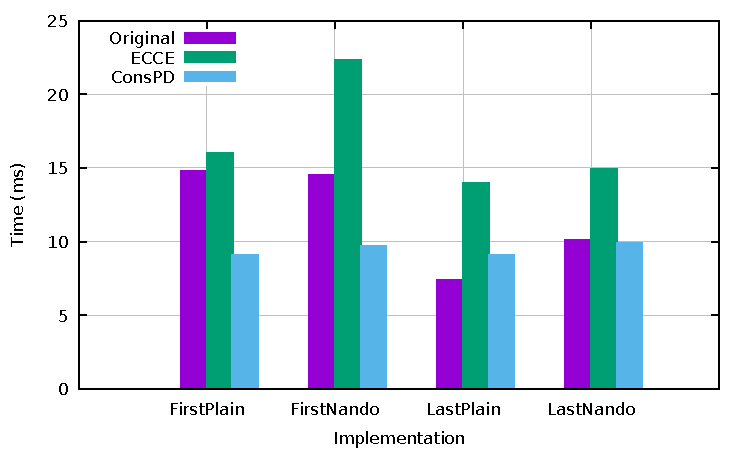
\includegraphics[width=\textwidth]{data/propEval/prop.pdf}
  \end{subfigure}
  \caption{Execution time of evalo}
  \label{fig:eval}
\end{figure}

Conservative partial deduction generates  programs with comparable performance for all four implementations, while the quality of \ecce specialization differs significantly.
\ecce worsens performance for every implementation as compared to the original program.
ConsPD do not worsen performance for any implementation.
Its effect is most significant for the implementations in which the boolean connectives are placed first within conjunctions.

\subsubsection{The Order of Answers}

It is important to note that different implementations of the same \mk relation produce answers in different orders.
Nevertheless, since \mk search is complete, all answers will be found eventually.
Unfortunately, it is not guaranteed that the first 1000 formulas generated with different implementations of \lstinline{eval$^o$} will be the same.
For example, $983$ formulas are the same among the first $1000$ formulas generated by the Original \emph{FirstPlain} relation and the same relation after the ConsPD transformation.
At the same time, only $405$ formulas are the same between the Original and \ecce \emph{LastNando} relations.

The reason why implementations differ so much in the order of the answers stems from the canonical search strategy employed in \mk.
Most \mk implementations employ \emph{interleaving} search~\cite{10.1145/1090189.1086390} which is left-biased.
It means that the leftmost disjunct in a relation is being executed longer than the disjunct on the right.
This property is not local which makes it very hard to estimate the performance of a given relation.

In practice it means that if a specializer reorders disjuncts, then the performance of relations after specialization may be unpredictable.
For example, by putting the disjuncts of the \lstinline{eval$^o$} relation in the opposite order, one produces a relation which runs much faster than the original, but it generates completely different formulas at the same time.
Most of the first 1000 formulas in this case are multiple negations of a variable, while the original relation produces more diverse set of answers.
Computing a negation of a formula only takes one recursive \lstinline{eval$^o$} call thus finding such answers is faster than conjunctions and disjunctions.
Meanwhile, the formulas generated by the reordered relation are less diverse and may be of less interest.

Although neither \ecce nor ConsPD reorder disjuncts, they remove disjuncts which cannot succeed.
Thus they influence the order of answers and performance of relations.
We believe that, in general, it is not possible to guarantee the same order of answers after specialization.
Exploring how different specializations influence the execution order is a fascinating direction for future research.


\subsection{Typechecker-Term Generator}

This relation implements a typechecker for a tiny expression language.
Being executed in the backward direction it serves as a generator of terms of the given type.
The abstract syntax of the language is presented below.
The variables are represented with de Bruijn indices, thus let-binding does not specify which variable is being bound.

\[\begin{array}{lllll}
  type \ term = &\ BConst \ of \ Bool &| \ IConst \ of \ Int &| \ Var \ of \ Int & \\
  & | \ term + term &| \ term * term &| \ term = term &| \ term < term \\
  &| \ \underline{let} \ term \ \underline{in} \ term
  &\multicolumn{2}{l}{| \ \underline{if} \ term \ \underline{then} \ term \ \underline{else} \ term} &
\end{array}\]

The typing rules are straightforward and are presented below.
Boolean and integer constants have the corresponding types regardless of the environment.
Only terms of type integer can be summed up, multiplied or compared by less-than operator.
Any terms of the same type can be checked for equality.
Addition and multiplication of two terms of suitable types have integer type, while comparisons have boolean type.
If-then-else expression typechecks only if its condition is of type boolean, while both then- and else-branches have the same type.
An environment $\Gamma$ is an ordered list, in which the $i$-th element is the type of the variable with the $i$-th de Bruijn index.
To typecheck a let-binding, first, the term being bound is typechecked and is added in the beginning of the environment $\Gamma$, and then the body is typechecked in the context of the new environment.
Typechecking a variable with the index $i$ boils down to getting an $i$-th element of the list.

\begin{table}[!h]
  \setlength{\tabcolsep}{0.4cm}
  \centering
  \begin{tabular}{c c c}
    \infer[]{\Gamma \vdash IConst \ i : Int}{} &
    \infer[]{\Gamma \vdash BConst \ b : Bool}{}  &
    \infer[\Gamma \lbrack v \rbrack \equiv \tau]{\Gamma \vdash Var \ v : \tau}{} \vspace{0.5cm}
    \\
    \infer[]{\Gamma \vdash t + s : Int}{\Gamma \vdash t : Int, \Gamma \vdash  s : Int}  \vspace{0.5cm} &
    \infer[]{\Gamma \vdash t = s : Bool}{\Gamma \vdash t : \tau, \Gamma \vdash  s : \tau} &
    \infer[]{\Gamma \vdash \underline{let} \ v \ b : \tau}{\Gamma \vdash v : \tau_v, \ (\tau_v :: \Gamma) \vdash b : \tau}
      \\

      \infer[]{\Gamma \vdash t * s : Int}{\Gamma \vdash t : Int, \Gamma \vdash  s : Int}  &
    \infer[]{\Gamma \vdash t < s : Bool}{\Gamma \vdash t : Int, \Gamma \vdash  s : Int} \vspace{0.5cm} &
      \infer[]{\Gamma \vdash \underline{if} \ c \ \underline{then} \ t \ \underline{else} \ s : \tau}{\Gamma \vdash c : Bool, \Gamma \vdash t : \tau, \Gamma \vdash s : \tau}
  \end{tabular}
\end{table}


We compared two implementations of these typing rules.
The first one is obtained by unnesting of a functional program as described in~\cite{lozov2019relational} (\emph{Generated}).
It is worth noting that the unnesting introduces a lot of redundancy in form of extra unifications and thus creates programs which are very inefficient.
Thus we contrast this implementation with the program hand-written in \oc (\emph{Hand-written}).
Each implementation has been specialized with ConsPD and \ecce.
We measured the time needed to generate 1000 closed terms of type integer (see Fig.~\ref{tbl:type}).


\begin{figure}[!h]
  \begin{subfigure}[c]{0.55\textwidth}
    \centering
    \begin{tabular}{c||c|c|c}
                          & Original & \ecce & ConsPD  \\ \hline\hline
      \emph{Hand-written} & 0.92s    & 0.22s & 0.34s   \\ \hline
      \emph{Generated}    & 11.46s   & 0.38s & 0.29s
      \end{tabular}
  \end{subfigure}
  \hfill
  \begin{subfigure}[c]{0.45\textwidth}
    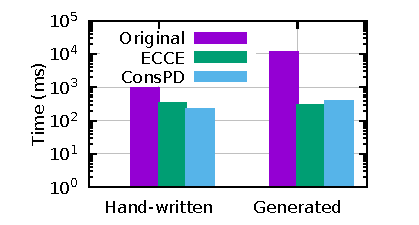
\includegraphics[width=\textwidth]{data/lTypecheck/ltypelog.pdf}
  \end{subfigure}
  \caption{Execution  time of generating 1000 closed terms of type Integer}
  \label{tbl:type}
\end{figure}

As expected, the generated program is far slower than the hand-written.
The principal difference between these two implementations is that the generated program contains a certain redundancy introduced by unnesting.
For example, typechecking of the sum of two terms in the hand-written implementation consists of a single conjunction (see Listing~\ref{type:hand}) while the generated program is far more complicated and also uses a special relation \lstinline{typeEq$^o$} to compare types (see Listing~\ref{type:gen}).

\begin{figure*}[!h]
  \centering
    \begin{lstlisting}[label={type:hand}, caption={A fragment of hand-written typechecker}, captionpos=b, frame=tb]
  let rec typecheck$^o$ gamma term res = conde [
    ...
    fresh (x y) ((term === x + y /\
       typecheck$^o$ gamma x ^(Some Integer) /\
       typecheck$^o$ gamma y ^(Some Integer) /\
       res === ^(Some Integer)));
    ...]
    \end{lstlisting}
\end{figure*}


\begin{figure*}[!t]
  \centering
    \begin{lstlisting}[label={type:gen}, caption={A fragment of generated typechecker}, captionpos=b, frame=tb]
let rec typecheck$^o$ gamma term res = conde [
  ...
  fresh (x y t1 t2) ((term === x + y /\
    conde [
      typecheck$^o$ gamma x ^None       /\ res === ^None;
      typecheck$^o$ gamma x ^(Some t1) /\
        typecheck$^o$ gamma y ^None     /\ res === ^None;
      typecheck$^o$ gamma x ^(Some t1) /\  typecheck$^o$ gamma y ^(Some t2) /\
        typeEq$^o$ t1 Integer ^true     /\ typeEq$^o$ t2 Integer ^true /\
        res === ^(Some Integer);
    ])
  ...]
    \end{lstlisting}
\end{figure*}

Most of the redundancy of the generated program is removed by specialization with respect to the known type of the term.
This is why both implementations have comparable speed after specialization.
\ecce shows bigger speedup for the hand-written program than ConsPD and vice versa for the generated implementation.
We believe that this difference can be explained by too much unfolding.
\ecce performs a lot of excessive unfolding for the generated program and only barely changes the hand-written program.
At the same time ConsPD specializes both implementations to comparable programs performing average amount of unfolding.
This shows that the heuristics we presented gives more stable, although not the best, results.

% У заключения нет номера главы
\clearpage

\section*{Заключение}
В ходе данной работы получены следующие результаты. 
\begin{itemize}
  \item Изучена предметная область: методы обработки встроенных языков и алгоритм обобщённого синтаксического анализа RNGLR.
  \item Разработан алгоритм синтаксического анализа динамически формируемых выражений, поддерживающий работу с произвольными входными графами.
  \item Доказана корректность алгоритма:
  \begin{itemize}
    \item алгоритм завершит работу для любых входных данных;
          %для любой входной детерминированной контекстно-свободной грамматики и 
          %произвольного входного графа алгоритм завершит свою работу;
    \item для любой цепочки из входного множества, выводимой в эталонной грамматике G, в SPPF содержится её дерево вывода в G; при этом никакие другие деревья не содержатся в SPPF.
          %для любой цепочки, которую может породить автомат (которая содержится 
          %в регулярном множестве), выводимой в рассматриваемой грамматике G, в 
          %SPPF содержится её дерево вывода в G, при этом не содержится никаких 
          %других деревьев.
  \end{itemize}
  \item Выполнена реализация алгоритма на языке программирования F\# в рамках исследовательского проекта YaccConstructor.
  \item Проведена апробация: регрессионное тестирование, тестирование производительности и тестирование на реальных данных.
  \item Исходный код проекта YaccConstructor можно найти на сайте \url{https://github.com/YaccConstructor/YaccConstructor}, автор принимал участие под учётной записью kajigor.
\end{itemize}

В дальнейшем планируется изменить алгоритм таким образом, чтобы помимо 
построения леса разбора всех корректных выражений осуществлялся бы также поиск ошибочных выражений и сообщение о них. Также необходимо произвести теоретическую оценку сложности алгоритма. Предложенный алгоритм планируется внедрить в инструмент по реинжинирингу информационных систем.  

\bibliographystyle{ugost2008ls}
\bibliography{diploma.bib}
\end{document}
